
\documentclass[a4paper,14pt,russian]{extreport}	%A4 бумага, 14 кегль, русский язык 
\usepackage{extsizes}
\usepackage[onehalfspacing]{setspace} % поулторный интервал %https://proft.me/2013/06/9/latex-ukazanie-mezhstrochnogo-intervala

\usepackage{cmap} % для кодировки шрифтов в pdf
\usepackage[T2A]{fontenc}
%\usepackage{pscyr}
%\usepackage{graphicx} % для вставки картинок
\usepackage{mathptmx} %поддержка textbf
\usepackage{makecell}
\usepackage{textcomp}
\usepackage{multirow} % улучшенное форматирование таблиц
\usepackage{ulem} % подчеркивания

%полужирный шрифт http://tostudents.ru/2009/12/08/smena-shriftov-v-latex-tekst-i-formuly/
\renewcommand{\rmdefault}{ftm} % Times New Roman
\usepackage[utf8]{inputenc}%включаем свою кодировку: koi8-r или utf8 в UNIX, cp1251 в Windows
%\usepackage[]{babel}	%больше поддержки русского языка 
\usepackage[english,russian, russianb]{babel}%используем русский и английский языки с переносами
\usepackage{amssymb,amsfonts,amsmath,mathtext,cite,enumerate,float} %подключаем нужные пакеты расширений

\usepackage[pdftex]{graphicx} %хотим вставлять в диплом рисунки?
\usepackage{cmap} % Улучшенный поиск русских слов в полученном pdf-файле
%\graphicspath{{images/}}%путь к рисункам
\usepackage{fancyhdr}%оформление нумерации 
\usepackage{tableof} %поддержка табличек
\usepackage{mathptmx}%
\usepackage{anyfontsize}% http://texblog.org/2012/08/29/changing-the-font-size-in-latex/
\usepackage{t1enc}%
\usepackage{cite}
\usepackage{graphicx}
\usepackage{longtable}
\usepackage{lscape}
\graphicspath{{Images/}} %http://dkhramov.dp.ua/Comp.TexIncludeGraphics#.WwLdJa3sTMU
\DeclareGraphicsExtensions{.pdf,.png,.jpg} %http://dkhramov.dp.ua/Comp.TexIncludeGraphics#.WwLdJa3sTMU
 %https://tex.stackexchange.com/questions/17734/cannot-determine-size-of-graphic
\makeatletter
\renewcommand{\@biblabel}[1]{#1.} % Заменяем библиографию с квадратных скобок на точку:
\makeatother

\usepackage{geometry} % Меняем поля страницы
%QUEST: 3cm или 2 ? Ес\usepackage{cmap} % Улучшенный поиск русских слов в полученном pdf-файлели 3, придется менять форматирование заголовка 
\geometry{left=3cm}% левое поле
\geometry{right=2cm}% правое поле
\geometry{top=2cm}% верхнее поле
\geometry{bottom=2cm}% нижнее поле


\renewcommand{\theenumi}{\arabic{enumi}}% Меняем везде перечисления на цифра.цифра
\renewcommand{\labelenumi}{\arabic{enumi}}% Меняем везде перечисления на цифра.цифра
\renewcommand{\theenumii}{.\arabic{enumii}}% Меняем везде перечисления на цифра.цифра
\renewcommand{\labelenumii}{\arabic{enumi}.\arabic{enumii}.}% Меняем везде перечисления на цифра.цифра
\renewcommand{\theenumiii}{.\arabic{enumiii}}% Меняем везде перечисления на цифра.цифра
\renewcommand{\labelenumiii}{\arabic{enumi}.\arabic{enumii}.\arabic{enumiii}.}% Меняем везде перечисления на цифра.цифра
\addto\captionsrussian{\def\refname{Список используемой литературы}}
\renewcommand{\rmdefault}{ftm}
%NB: три команды ниже переопределяют некотрые шрифты  и дают поддержку жирного и прочиах текстов https://www.linux.org.ru/forum/general/4219163
\renewcommand{\rmdefault}{cmr} % Шрифт с засечками
\renewcommand{\sfdefault}{cmss} % Шрифт без засечек
\renewcommand{\ttdefault}{cmtt} % Моноширинный шрифт
\renewcommand*\thesection{\arabic{section}}
    
\begin{document}
	\numberwithin{equation}{subsection} %Стилистика нумерования уравненений в \begin{equation} \label{name:\d}. Тут -- номер главы.сабсекция.номер_уравнения_с_лэйблом_name
	% https://en.wikibooks.org/wiki/LaTeX/Advanced_Mathematics#Equation_numbering
	%http://fkn.ktu10.com/?q=node/6860
	\renewcommand{\bibname}{Список использованной литературы}
	%\pagestyle{empty} % нумерация выкл.
	    \begin{titlepage}
    \newpage
	\pagestyle{empty} % нумерация выкл.
    \begin{center}
    \normalsize МИНИСТЕРСТВО ОБРАЗОВАНИЯ И НАУКИ РОССИЙСКОЙ ФЕДЕРАЦИИ\\ 
    \small  {Федеральное государственное автономное образовательное учреждение высшего образования} 
    \large \textbf{<<Крымский  федеральный  университет имени В. И. Вернадского>>} \\  \vspace{2mm}
    Таврическая академия (структурное подразделение ) \\
    \vspace{2mm}
    Факультет математики и информатики \\
    \vspace{2mm}
    Кафедра прикладной математики 
    \end{center}
    \vspace{3em}

    \begin{center}
	\normalsize Консманов Алексей Витальевич \\
    \LARGE \textbf{Сохранение тайны связи в условиях новых цифровых угроз} \\
    \vspace{1em}
    \normalsize Курсовая работа 
    \end{center}

    \vspace{1em}
    
    \begin{center}
    	\begin{tabbing}	%http://www.intuit.ru/studies/courses/1137/137/lecture/3835%3Fpage%3D5
    		\hspace{3cm}Обучающегося \hspace{3cm} \textbf{3 курса}\\ %Быдлокод?
    		\hspace{3cm}Направления подготовки \hspace{7mm}  \textbf{01.03.04}\\
    		\hspace{3cm}Форма обучения \hspace{26mm} \textbf{очная}
    	\end{tabbing}
    
	\vspace {3em}
    \flushleft Научный руководитель \hspace{20mm}  старший преподаватель 
    
    \hspace{75mm}кафедры прикладной математики  
    
    
    \hspace{75mm}В. А. Лушников
	\end{center}
    \vspace{\fill}

    \begin{center}
    Симферополь 2018
    \end{center}

    \end{titlepage}
% это титульный лист

	\tableofcontents % это оглавление, которое генерируется автоматически
	\thispagestyle{empty}%отключает нумерование страниц до введения включительно 
	%\addcontentsline{toc}{section}{Введение}% будет костыльно выглядеть
	\newpage
\parindent=1cm %красная строка? 
\begin{center}
	\addcontentsline{toc}{section}{Введение} %Убираем номер , даём имя в оглавлении 
	\section*{Введение} %сам текст заголовка 
	\pagestyle{plain} % нумерация выкл.
	\setcounter{page}{3} % начать нумерацию с номера тр
\end{center}

Актуальность работы  связана с возросшим числом новых угроз в области защиты личных данных, участившимися атаками частных лиц, группировок и специальных ведомств иностранных государств против частных лиц с целью получения частной информации, анализа полученных личных данных   и использования для шантажа атакуемых лиц, продажи или другого выгодного обмена, а также  в иных противозаконных целях. 

Целью данной работы является %EDIT: сделать это в виде списка с пунктами?
 анализ новых цифровых угроз, возникших в последнее десятилетие в связи с бурным развитием информационных технологий, за которым не последовал соразмерный рост знаний пользователей цифровых систем, используемые кибер-преступниками методы анализа и атаки на частные данные, правовой аспект защиты личной переписки, способы борьбы с угрозами  в рамках существующего программного обеспечения, %EDIT: заменить на ПО и создать список используемых сокращений до введения?
 сравнительный анализ существующих продуктов, разработка и реализация собственных алгоритмов для сохранения тайны личной переписки. 	 %введение
	\parindent=1cm %красная строка

\begin{center}
		
		\section{Мультиагентное моделирование системы поддержки принятия решений в составе системы противоракетной обороны}
		
\end{center}

\subsection{Описание системы ПРО} 

Как правило, процесс противоракетной обороны (далее ПРО) состоит из последовательности этапов, включающих ранее обнаружение, отслеживание, распознавание, принятие решения и непосредственный перехват цели, достигаемый посредством взаимодействия всех компонентов системы ПРО (далее СПРО). 

Не вдаваясь в технические подробности и устройство составных компонентов СПРО, отметим только сами компоненты и функции, выполняемые этими компонентами:

\begin{itemize}
	\item Радар раннего обнаружения фиксирует факт запуска ракет и получает приблизительные данные о положении и скорости;
	\item отслеживающий радар <<ведёт>> ракету-перехватчик до завершения перехвата или промаха, получая инструкции из командного центра и передавая их ракете-перехватчику;
	\item командный центр выполняет роль коммуникационного звена и центра обработки информации; производит оценку траектории ракеты, на основании  данных от радара раннего обнаружения; отправляет информацию отслеживающему радару;  создание (генерация) плана перехвата ракеты и отправка его ракете-перехватчику в подходящий момент времени;
	\item ракета-перехватчик выполняет задачу перехвата и способна к ограниченному маневрированию.
\end{itemize} 

Очевидно, что для полного цикла работы СПРО необходима и ракета-цель. 


\subsection{Агентное моделирование и понятие <<агента>>}


Понятие <<агент>> не является строго установленным, но в общем случае можно говорить об <<агенте>> как о сущности, имеющей активность, автономное поведение, способность к самостоятельному приему решений в соответствии  с некоторой заранее заданной совокупностью правил, способность к взаимодействию  с окружающей средой и другими агентами (если такие существуют в рамках модели). Мультиагентные же модели в свою очередь используют множества таких агентов для построения процессов, где поведение системы возникает как следствие взаимодействия множества агентов, а не поведение системы описывает поведение каждого агента, т.е происходит моделирование <<снизу вверх>>.

В рамках данной работы агент будет иметь следующую структуру:
\begin{itemize}
	
	\item сенсор -- получает информацию из внешнего мира в рамках радиуса восприятия;
	\item контроллер -- ядро агента, состоящее из базы априорных знаний, базы правил и системы  принятия решений (СПР)
	\item пр\'{и}вод -- исполняющий компонент агента, ответственный за применение обратной связи к окружающей среде  

\end{itemize}

Примерная структура агента описана схематично на рис. 1.

\begin{figure*}[h!]
	\centering{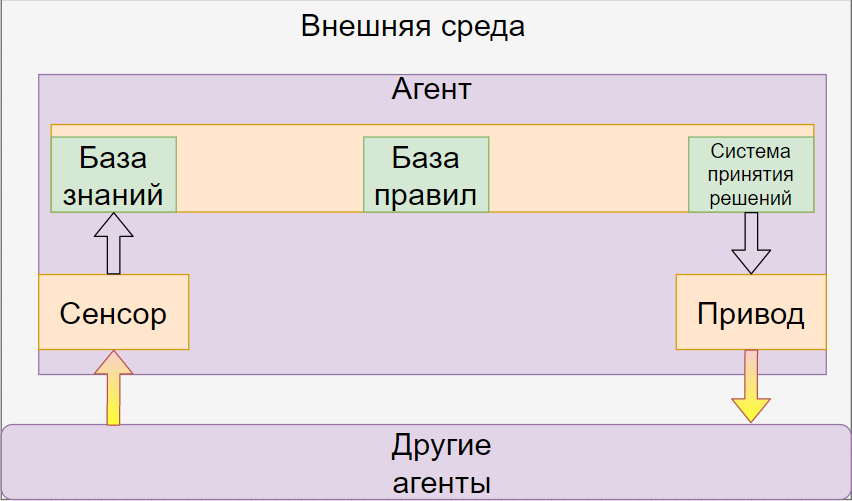
\includegraphics[scale=0.85]{GeneralAgentSchema.png}}
	\caption{Схематическое описание структуры агента и среды}.
\end{figure*} 

Согласно приведенной на рис. 1 схеме, агент способен принимать решения в соответствии с логическими  высказываниями, хранящимися в его базах и / или на основании результатов вычислений. СПР является самой важной частью агента, т.к именно она отвечает за принятие решений. СПР работает по следующему алгоритму: построение модели ограничений на основании данных, полученных из сенсора; выбор наиболее подходящего поведения на основании базы правил и априорной базы знаний.  В целом, СПР может имплементировать механизм дополнительного обучения, позволяющий изменять существующие правила и знания и / или добавлять новые.  

В рамках рассматриваемой в данной работы СПРО, компоненты моделируются с использованием мультиагентного подхода, то есть каждый компонент системы представляет собой агент. СПР решений командного центра СПРО будет генерировать планы перехвата цели динамически, используя для этого данные с радаров обнаружения и вычислительный эксперимент в рамках СПРО. Агенты СПРО показаны на рис. 2. Компоненты одинакового цвета имеют одинаковые возможности. 

\begin{figure*}[h!]
	\centering{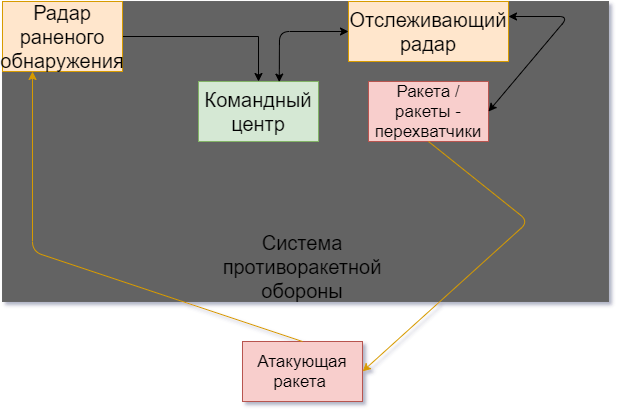
\includegraphics[scale=0.85]{BmdsSchema.png}}
	\caption{Схематическое описание структуры СПРО, связей в ней и воздействия атакующей ракеты}.
\end{figure*} 


\pagebreak


\subsubsection{Агент <<командный центр>>}

Агент <<командный центр>> выполняет назначение конкретной ракеты-перехватчика на цель и посылает инструкции о запуске. Ниже представлена таблица знаний данного агента.

% Please add the following required packages to your document preamble:
% \usepackage{longtable}
% Note: It may be necessary to compile the document several times to get a multi-page table to line up properly
\begin{longtable}{|l|p{0.4\linewidth}|}
	\multicolumn{2}{l}{} \\
	\hline
	Свойство & Значение \\ \hline
	\endfirsthead
	%
	\endhead
	%
	Позиция командного центра (координаты)		& 	широта, долгота, высота	\\ \hline
	Позиция ракеты-перехватчика					&	широта, долгота, высота	\\ \hline 
	Угол наклона ракеты-перехватчика			&	вычисляется с помощью  формул сферической геометрии	     \\ \hline
	Время запуска ракеты-перехватчика			&	вычисляется в рамках решения задачи Ламберта          \\ \hline
	Время подлета ракеты-перехватчика к цели 	&	вычисляется в рамках решения задачи Ламберта         \\ \hline
	Вероятность перехвата						&  	вычисляется ракетой-перехватчиком	     \\ \hline 
	\caption{Таблица знаний командного центра}
	\label{tab:command_center_parameters}\\
\end{longtable}


Правила командного центра включают правила оценки угроз и правила выбора ракеты перехватчика. Эти правила поддерживаются нижеописанной моделью принятия решений.

\textbf{Вычислительная модель назначения ракеты-перехватчика}.
Эта модель генерирует план-назначение ракет-перехватчиков. Для этого используются  местоположение, тип и количество доступных ракет-перехватчиков, уровень угрозы и количество атакующих ракет и время их определения. 

\textbf{Вычислительная модель для точки перехвата}.
Точка перехвата определяется как точка, находящаяся на траектории атакующей ракеты и ближе всего к максимальной высоте ракеты-перехватчика, что позволит запускать дополнительные ракеты в случае неудачи. В свою очередь, траектория атакующей ракеты определяется посредством анализа данных, накапливаемых радаром раннего обнаружения и отслеживающим радаром. Эти данные являются массивом, где каждый элемент имеет вид  <<пара \{координаты, время\} >>.  Максимальная высота, достигаемая ракетой-перехватчиком вычисляется из характеристик этой ракеты, но в данной работе для упрощения вычислений является свойством самой ракеты.

\textbf{Вычислительная модель определения времени запуска ракеты-перехватчика}.
Пусть $T_L$ -- время запуска ракеты-перехватчика; $T_e$ -- момент времени, когда цель окажется в точке перехвата; $T_f$ -- время полета ракеты-перехватчика к точке перехвата; $T_p$ -- время подготовки ракеты-перехватчика к запуску, в данной работе полагаемое константной (однако, можно предположить, что в реальности этот параметр будет вести себя как  модуль квадратичной функции, зависящей от кол-ва подготовленных ракет-перехватчиков, с положительным старшим коэф-том и нулевым дискриминантом, возникающим при приравнивании этой функции нулю). Тогда $T_L = T_e - T_f - T_p$.

\textbf{Модель вычисления угла наклона}
Пусть $A$ -- точка запуска ракеты-перехватчика, $B$ -- предполагаемая точка перехвата, северный полюс --  $C$. Тогда эти три точки вместе с геоцентрической точкой $o$ (центр Земли) формируют сферический треугольный конус; $A, B, C$ представляют угол между двумя гранями, а $a,b,c$  -- геоцентрический угол между двумя точками. Получаем, что угол наклона $\theta_f=arccos(cos(a) \cdot cos(b)+sin(a) \cdot sin(b) \cdot cos(c))$, где 
$a=90-T_{Lat}, b=90-L_{Lat}, C=T_{Lon}-L_{Lon}$, где $L_{Lon}$, $L_{Lat}$ и  $T_{Lon}$, $T_{Lat}$ представляют собой долготу и широту точки запуска и целевой точки перехвата.

\textbf{Модель вычисления параметров уничтожения ракеты-цели}.
Установив начало координат в центр Земли и положив $OX$ как ось, соединяющую центр Земли и точку пуска ракеты, получим полярную систему координат. Обозначим $r_1$, $r_2$, вектор точки запуска и вектор перехвата из геоцентрической точки начала координат; $\theta_f$ -- угол наклона получаемый как $\theta_f = arccos(\frac{r1 \cdot r2}{|r1| \cdot |r2|})$; $\gamma$ -- угол наклона траектории получаемый как $\gamma = \frac{\pi - \theta_f}{4}$ при движении по траектории с минимальной энергией; $\mu$ -- гравитационная константа.    Согласно уравнению Ламберта, скорость перехвата ракеты $V_s$ удовлетворяет условию 
$V_s = \sqrt{\frac{|r_2|(1-cos \theta_f)\mu}{|r_1|^2 \cdot cos(\gamma ^ 2) - |r_2| \cdot  cos(\theta_f + \gamma) \cdot cos \gamma}}$.
Так как траектория полеты -- эллипс, то время полеты ракеты рассчитывается как
$t_f = \frac{|r_1|}{V \cdot cos(\gamma) (\frac{tan(\gamma) (1-cos \theta_f) + (1-\lambda sin \theta_f)}{(2-\lambda)  \frac{|r_1|}{|r_2|}})} + \frac{2cos \gamma}{\lambda ((2/ \lambda) - 1)^{1.5}} arctan \frac{((2-\lambda) - 1) ^ {0.5}}{cos \gamma \cdot ctg(\frac{\theta_f}{2}) - sin \gamma}$, где $\lambda = |r_1| \cdot \frac{V^2}{\mu} $. 


\begin{figure*}[h!]
	\centering{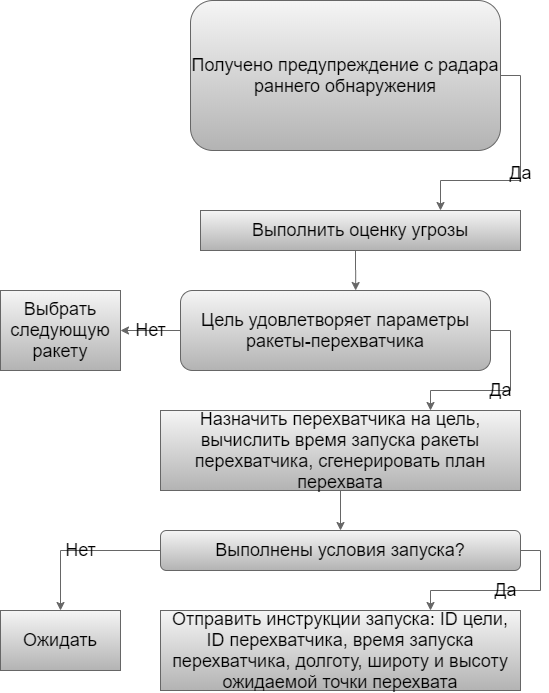
\includegraphics[scale=0.85]{CommandCenterInstruction.png}}
	\caption{Блок схема принятия решения командным центром}.
\end{figure*} 


\subsubsection{Агент <<ракета>>}

В терминах ООП,  <<ракета>> является абстрактным базовым классом, от которого наследуются атакующая ракета и ракета-перехватчик. База его знаний хранит данные, необходимые для вычисления траектории и включает позицию и скорость ракеты, т.е. в каждый момент времени известна широта, долгота, высота и скорость ракеты. 

\begin{figure*}[h!]
	\centering{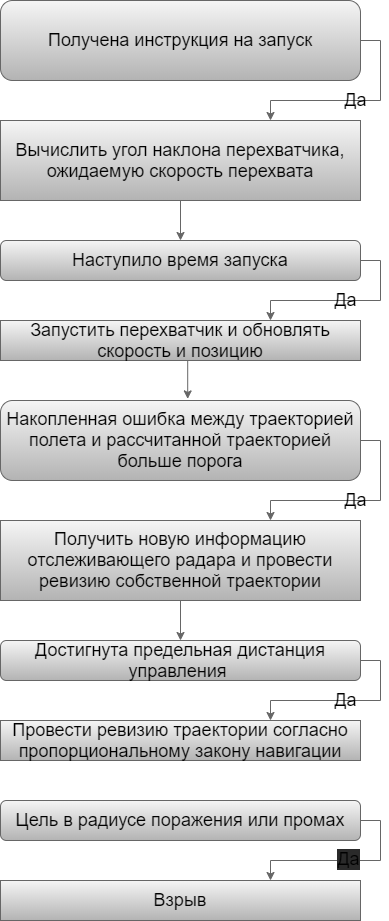
\includegraphics[scale=0.6]{RocketInstruction.png}}
	\caption{Блок схема принятия решения ракетой-перехватчиком}.
\end{figure*} 


\subsubsection{Агент <<радар>>}

Как и в прошлом случае, <<радар>> является абстрактным базовым классом. База знаний радара содержит преимущественно данные для вычисления радиуса радарного покрытия и угла покрытия.   Правила радара включают правила обнаружения и правила предсказания движения ракеты. Правила обнаружения вычисляют область радарного покрытия через радарное уравнение и считается, что любой объект в области радарного покрытия мгновенно обнаруживается при первом сканировании, т.е. в рамках данной работы не рассматриваются цели с активным подавлением радаров или постановкой помех; правила предсказания отсылают информацию в командный центр если объект был замечен хотя бы трижды. 

Полагая, что ракета цилиндрической формы, обозначим $r$ -- радиус ракеты, $h$ -- длина боеголовки, $\lambda$  -- длина волны сигнала радара, $h_1, h_2, h_3$ -- длина двигателей этапа с соответствующим номером. Эффективный поперечник рассеяние (ЭФР) зависит также от угла между радаром и проекций  движения ракеты на  OY, обозначенным как $\theta$ Тогда эффективный поперечник рассеяния ракеты-цели согласно эмпирической формуле равен $R = 2 \pi r (\frac{h_1^2}{\lambda} + \frac{h_2^2}{\lambda} + \frac{h_3^2}{\lambda} + \frac{4}{9 \lambda h} \cdot \sqrt{(r^2+h^2)^3} ) * cos \theta$.

\begin{figure*}[h!]
	\centering{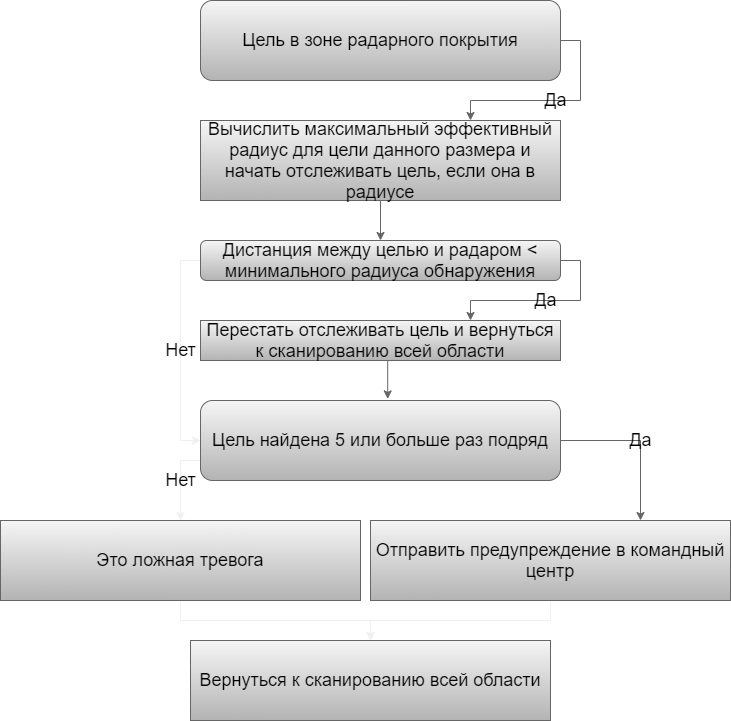
\includegraphics[scale=0.6]{RadarInstruction.png}}
	\caption{Блок схема принятия решения радаром раннего обнаружения}.
\end{figure*} 


\subsection{Система обозначений  и ограничений для алгоритма}

Введем систему обозначений, которые в дальнейшем будут использованы для описания компонентов в алгоритме перехвата целей. 


\begin{longtable}{|l|p{0.4\linewidth}|}
	\multicolumn{2}{l}{} \\
	\hline
	Обозначение & Определение \\ \hline
	\endfirsthead
	%
	\endhead
	%
	n		&	кол-во атакующих ракет-целей	\\ \hline
	j ($\in [0; n]$)		&	номер атакующей ракеты 	\\ \hline
	$T_j$	&	<<угроза>> атакующей ракеты №j	\\ \hline
	$R_j$	&	время на перехват ракеты №j как расстояние от размещения перехватчиков до цели \\ \hline
	$C_j$	&	фактор возможного вмешательства командира	\\ \hline
	$D_j$	&	расстояние от атакующей ракеты №j до цели (цель общая для всех ракет)	\\ \hline
	$S_j$	&	максимальная скорость ракеты №j	\\ \hline
	m		& 	кол-во ракет перехватчиков	\\ \hline
	i ($\in [0; m]$)		&	номер ракеты-перехватчика \\ \hline
	$V_i$	&	<<цена>> ракеты-перехватчика №i	\\ \hline
	$w_k$	&	массив (вектор) специальных весов \\ \hline
	$P_{ij}$ ($P_{ij} \in [0; 1]$)	&	вероятность перехвата ракетой $i$ ракеты $j$	\\ \hline
	$x_{ij}$	&	Булеан, указывающий назначена ли ракета $i$ на ракету $j$	\\ \hline 
	\caption{Символы, используемые для обозначения компонентов алгоритма}
	\label{tab:algorithm_defenitions}\\
\end{longtable}

Отбросим ситуации, где n или m равны 0, т.к. это автоматически приводит к бесконечному множеству решений или пустому множеству решений соответственно. Также заметим, что в рамках этой работы m $\ge$ n.

При решении задачи должны соблюдаться следующие ограничения:

1.Для обеспечения безопасности целей, атакуемых ракетами, необходимо назначить хотя бы одну ракету-перехватчик на каждую цель и приоритет по кол-ву ракет и очередности назначения должен отдаваться ракетам с максимальной <<угрозой>>  и назначаться должны ракеты с минимальной <<стоимостью>>, что позволит избежать быстрого расхода самых <<лучших ракет-перехватчиков>>. Это можно выразить таким фитнесом:
$\sum_{j=1}^{n} \sum_{i=1}^{n}  \frac{T_{j}P_{ij} x_{ij}}{V_{i}x_{ij}}$. 
\newline
2. Генерация плана перехвата зависит от оперативности и качества данных, приходящих с радара. Хорошообнаружимая ракета лучше отслеживается и должна иметь более высокий приоритет.  
\newline
3. Приоритет перехвата также отдается ракетам, более близким к обороняемым целям.
\newline
4. Предпочтительно перехватывать ракеты с более высокой скоростью.
\newline
5. Вмешательство командира, основанное на эмпирическом внешнем знании играет максимальную роль.
\newline
С учетом вышеизложенного, фитнес может быть описан следующим образом 
$\sum_{j=1}^{n}\sum_{i=1}^{m} \frac{P_{ij} \prod_{k=1}^{3}w_k T_j   S_j   C_j}{\prod_{l=4}^{6} w_l V_i x_{ij}  R_j D_j}$.

Для увлечения адаптируемости,  положим $w_x = 1, x \in [1; 6] $ 
\newpage % следующая глава с новой страницы
	\parindent=1cm %красная строка

\begin{center}
		
		\section{Алгоритм роя частиц  переменной окрестности  с отрицательным отбором и его применение}
		
\end{center}

\subsection{Общая идея алгоритма}

Метод роя частиц (МРЧ) использует множество частиц, каждая из которых представляет потенциальное решение и для каждой частицы можно посчитать фитнес-функцию, служащую для отбраковки худших решений. Изначально множество частиц инициализируется случайными значениями, однако важно, что каждая частица, являющая вектором, должна иметь многомерное равномерное распределение внутри своих значений. Текущая позиция частицы записывается $n$-мерным вектором и обозначается как $X=(X_1,...,X_n)$. i-ый элемент  частицы  в поисковом пространстве S обозначается как $X_i=$ $\begin{bmatrix}
	x_{i1} \\
	
	\vdots \\
	
	x_{iD}
\end{bmatrix}$; текущая скорость частицы обозначается как $V_i=$ 
$\begin{bmatrix}
V_{i1} \\ 

\vdots \\

V_{iD}
\end{bmatrix}$ ; локальная лучшая позиция $P_i$ = $\begin{bmatrix}
P_{i1} 	\\ 

\vdots	\\

P_{iD}
\end{bmatrix}$; глобальное наилучшее решение обозначается как $P_g$ = $\begin{bmatrix}
P_{g1} \\
\vdots \\
P_{gD}	
\end{bmatrix}$. 

Обозначим через $w$ инерционный вес, позволяющий балансировку локального и глобального поиска; $k$ -- номер итерации; $V_{id}$ --скорость частицы $i$ в  $d$-ом пространстве; $r_1, r_2$ -- случайные вещественные числа, такие, что $0 \le r_i \le 1, r_i \in \mathbb{R}, i \in \{1,2\}$; $c_1, c_2$ -- неотрицательные константы, "факторы ускорения".   Скорость и позиция каждой частицы обновляются итеративно по следующей формуле: 
\begin{equation} \label{basic_velocity_and_postion_eq}
	V_{id}^{k} = wV_{id}^{k-1}+c_1r_1(P_{id}^{k-1}-X_{id}^{k-1}) + c_2 r_2(P_{gd}^{k-1} - X_{id}^{k-1}); \\
	X_{id}^{k} = X_{id}^{k-1} + V_{id}^{k}
\end{equation}
 . Для исключения невалидных решений, позиции и скорости частиц ограничены интервалами $[-X_{max}; X_{max}]$ и $[-V_{max}; V_{max}]$ соответственно.

Фитнес каждой частицы вычисляется на каждой итерации; новое значение фитнес-функции сравнивается с текущими локальной и глобальной лучшей позицией; если новое значение превосходит старое, то локальная лучшая позиция будет обновлена и затем среди локальных лучших позиций проводится поиск по максимум фитнес функции; если этот максимум превосходит фитнес функцию глобального лучшего решения, то глобальное лучшее решение заменяется локальным лучшим решением с указанным максимумом. Во избежание зацикливания алгоритма вводится произвольное достаточно большое число $T_{max}$, ограничивающее число итераций алгоритма; в рамках реализации данного алгоритма $T_{max}$ постепенно убывает, что отражает ограниченное время на принятие решения при все более близкой ракете-цели. В конце выполнения алгоритма, наступит ли он сам по достижению заданной точности ли будет прерван $T_{max}$, вектор $P_g$ содержит лучшее решение и представляет собой <<выходные данные>> данного алгоритма.


Общие идеи применения указанного выше алгоритма в этой работе похожи на таковые в %LITER: основа
и изложены далее. Во-первых, необходимо убедиться в  назначении адекватного кол-ва перехватчиков на одну цель. Для этого сгенерированная и/или обновленная частица должна обновляться по правилу замены повторяющихся элементов в этой частице. Также необходимо избежать выхода скорости частицы за границу $V_{max}$. Для выполнения двух предыдущих условий можно представить формулу \ref{basic_velocity_and_postion_eq} в виде 

\begin{equation} \label{advanced_velocity_and_postion_eq}
V^{k} = 
	\begin{cases}
		V_{max}, V^{k} > V_{max} \\
		V^{k}, V_{min} \le V^{k} \le V_{max} \\
		V_{min}, V^{k} < V_{min}
	\end{cases};
X^{k} = 
	\begin{cases}
		X_{max}, X^{k} > X_{max} \\
		X^{k}, X_{min} \le X^{k} \le X_{max} \\
		X_{min}, X^{k} < X_{min}
	\end{cases}
\end{equation}.  \\
В-третьих, для обеспечения более  равномерной сходимости, параметр $w$ будет убывать линейно по формуле: $w = w_{end} + (\frac{T_{max}-k}{T_{max}})(w_0-w{end})$. \\
В-четвертых, $c_1, c_2$ можно использовать не как константы, а переменные, обозначающие фактор самообучения и группового  обучения соответственно и изменяющиеся согласно формуле: 

\begin{equation}
	\begin{cases}
		c_1 = c_{1_{min}} + \frac{(c_{1_{max}} - c_{1_{min}}) k }{T_{max}} \\ 
		c_2 = c_{2_{min}} + \frac{(c_{2_{max}} - c_{2_{min}}) k }{T_{max}}
	\end{cases}
\end{equation}



Введем вспомогательную переменную $K$ -- фактор сужения, необходимый для улучшения сходимости алгоритма. Введем для этого дополнительную переменную $\phi = c_1 + c_2: \phi \ge 2$ и дополнительные обозначения: $N_r$ -- радиус окрестности, меняющийся в ходе итераций; $P_{id}^{k}$ -- собственное экстремальное значение частицы; $P_{N_{r}d}^{k}$ -- экстремальное значение соседа.  Тогда $K = \frac{2}{ \lvert 2 - \phi - \sqrt{\phi ^ 2 - 4 \phi} \rvert}$. С учётом этих нововведений  в практической реализации работы будет использована следующая формула для обновления скорости частицы:

\begin{equation}	\label{best_velocity_and_postion_eq}
	V_{id}^{k} = w V_{id}^{k} - c_1 r_1 (X_{id}^{k-1} - P_{id}^{k-1}) - c_2 r_2 (X_{id}^{k-1} - P_{N_{r}d}^{k-1})
\end{equation}.


Теперь опишем упомянутый в начале главы процесс <<отрицательный отбор>>. <<Отрицательный отбор>> позволяет оптимизировать процесс варьирования окрестности, необходимый чтобы избежать попадания алгоритма в локальный экстремум посредством  обновления некоторых частиц до тех пор, пока не достигнуто условие. Основная идея процесса заключается в итеративном обновлении частиц в соразмерно пропорции $R_u$ при сходимости алгоритма. В свою очередь, сходимость алгоритма в процессе его выполнения определяется фактом того, что сходство частиц больше некоторого предела сходства $T_{aff}$. Обозначим сходство частицы $p$ в $d$-ом измерении как $A_{pd}$, $P_{gd}$ -- глобальное экстремальное значение.  %TODO: добавит определение для x 
Сходство частицы $p$ в $d$-ом измерении описывается $A{pd} = 1 + \frac{|P_{gd} - x_{pd}|}{X_{min} - X_{max}}$

Также введем формулу для сходства $p$-ой частицы как среднее сходство всех размерностей: $A_{pd} =  \frac {\sum_{d=1}^{D} A_{pd}} {D}$.

Теперь опишем с помощью простой блок-схемы ниже алгоритм отрицательного отбора для каждой частицы. Заметим, что согласно этой блок-схеме, механизм отрицательного отбора будет задействован только при достижении частицей состояния, в котором  каждая  размерность частицы меньше $T_{aff}$.


\begin{figure*}[h!]
	\centering{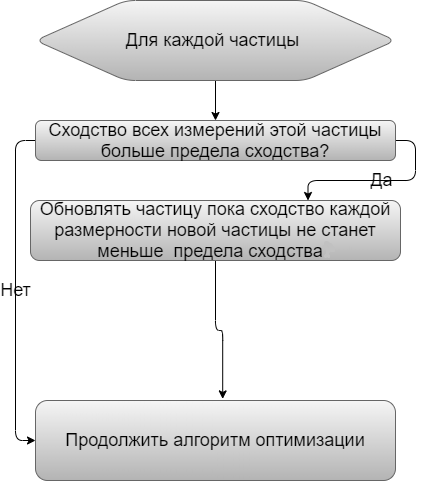
\includegraphics[scale=0.8]{NegativeSelectionProcess.png}}
	\caption{Блок-схема процесса <<отрицательного отбора>>}.
\end{figure*} 

После введения всех необходимых формул, изложения концепций и алгоритмов, играющих вспомогательную роль, опишем непосредственный алгоритм АРЯПОСОО. 

\begin{figure*}
	\centering{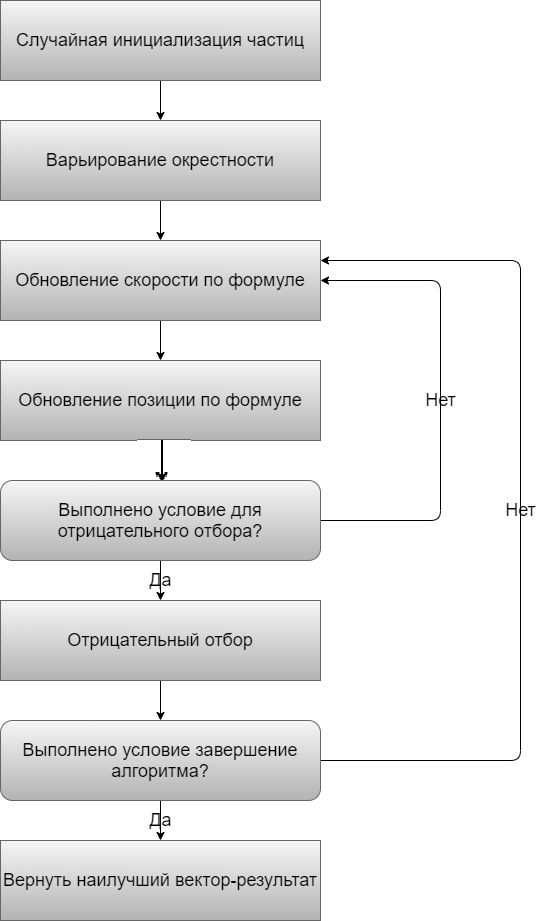
\includegraphics[scale=0.65]{MainAlgorithm.png}}
	\caption{Блок-схема процесса работы алгоритма роя частиц перемененной окрестности с отрицательным отбором}.
\end{figure*} 

\newpage 

\subsection{Реализация алгоритма и интеграция его в СПРО}.

Для быстроты написания, переносимости и использования готовых вспомогательных решений был выбран язык программирования Python 3.7.7. 

Для агентов был введен абстрактный базовый класс <<AbstractBaseClassAgent>> и  все используемые агенты являются экземплярами классов-наследников. Компоненты СПРО коммуницируют между собой с помощью веб-сокетов. Для симуляции передвижения ракет в трехмерном пространстве ракеты хранят на каждой итерации тройку координат внутри своего экземпляра, а <<сканирование>> радаром ракет происходит как анализ всех существующих в данный момент ракет с проверкой нахождения координат внутри области анализа. Возможно, такой подход не является полностью точным, но значительно экономит память и упрощает описание процесса <<сканирования>>; альтернативой данному подходу является создание трехмерного массива, дискретно описывающего пространство. 


Большой трудностью является реализация  одновременно происходящих параллельных событий. Обычно, в студенческих работах  для этого вводят некоторый порядок синхронных непараллельных действий и при этом предполагается, что вычисление этих действий происходит настолько быстро, что время исполнения кода ЦПУ не будет заметным. Однако, алгоритм АРЯПОСОО является затратным по времени, поэтому такой подход в данной работе невозможен.Вместо этого было решено использовать реальное параллельное выполнение кода. Проблемой Python в этой области явлвяется GIL ("Global Interpreter Lock"), однако, этого удалось избежать с использованием Thread- и ProcessPoolExecutor. Для реализации одновременности и параллельности каждый компонент выполняется в бесконечном цикле и <<спит>> 0.1 секунды после каждого своего <<тика>> (минимальная единица времени и действия); <<сон>>  с использованием time.sleep() необходим для создания пауз в выполнении кода процессором и переключении контекста выполнения, иначе  потребление ресурсов ЦПУ данным компонентом будет постоянным и вызовет задержки в переключении потока управления, когда число компонентов превысит число логических потоков ЦПУ, что в свою очередь создаст проблемы с симуляцией одновременности. Также заметим, что для быстрого освобождения ресурсов, поток ракеты при взрыве сразу останавливается и объект ракеты удаляется вручную.

Сама СПРО состоит из генератора атакующих ракет, который с заданной интенсивностью генерирует случайное нормально распределенное на заданному интервале кол-во атакующих ракет с разными параметрами полезной нагрузки, скорости и высоты (для простоты, этот компонент сразу генерирует ракеты находящиеся на этапе прохождения тропосферы), аналогичного генератора ракет-перехватчиков, имитирующего <<подвоз>>  ракет-перехватчиков в случайное время с интенсивностью, возрастающей по мере исчерпания запаса, трех радаров раннего обнаружения, 9 радаров отслеживания и переменного кол-ва ракет-перехватчиков, ограниченных сверху максимальной вместительностью склада, множества защищаемых объектов (программа завершает работу при полном уничтожении всех защищаемых объектов).
	\newpage
\parindent=1cm %красная строка
\addcontentsline{toc}{section}{Заключение} %Убираем номер , даём имя в оглавлении 
\section*{Заключение} %сам текст заголовка 

Разработанный и протестированный алгоритм имеет как преимущества, так и недостатки, рассмотрим их подробнее.


Преимущества: \\
\begin{itemize}
	\item Полная симуляция одновременно происходящих параллельных процессов;
	\item Минимальное, по сравнению с другими рассмотренными алгоритмами, число итераций;
	\item Возможность экспортировать данные в табличные процессоры для пост-обработки;
	\item Низкие затраты по памяти -- запущенное приложение при 10 активных ракетах-целях, 30 активных  ракетах-перехватчиках и 100 ракетах-перехватчиков на складе потребляет около 500 Мб ОЗУ;
	\item Высокие возможности распараллеливания алгоритма на критических участках -- потенциальный источник еще большей оптимизации исполнения алгоритма.
\end{itemize}

Недостатки: \\
\begin{itemize}
	\item Не самая высокая скорость сходимости среди рассмотренных;
	\item Симуляция параллельных событий требует процессора со значительным числом ядер и логических потоков, которые часто отсутствуют на встраиваемых системах, реально используемых в подобной технике. Так, описанное выше кол-во объектов создает около 50 процессов и более 100 потоков;
	\item Алгоритм рассматривает упрощенную схему полёта ракеты-цели и не учитывает возможных положений, допускающих оптимизацию процесса перехвата.
\end{itemize}

Были решены следующие задачи:

\begin{itemize}
	\item Описана СПРО для которой  построена модель и агенты, участвующие в ней;
	\item Описана система принятия решений и накладываемые на нее ограничения, алгоритм принятия решений;
	\item алгоритм принятия решений был реализован в виде ПО, протестирован и сравнён с другими подобными алгоритмами;
	\item были решены различные задачи, возникающие в области многоточечного программирования;
	\item были сделаны выводы о потенциале и возможностях развития развития данного алгоритма.
\end{itemize}

К сожалению, не удалось реализовать дополнительную цель и построить полноценный интерфейс приложения, позволяющий ввод-вывод данных и, самое важное, демонстрацию работы алгоритма посредством показа назначения ракет-перехватчиков на цели и непосредственно перехватом.

Несмотря на неидеальные параметры работы алгоритма, он всё же демонстрирует высокую скорость исполнения. Отметим, что как сам алгоритм АРЯПОСОО, так и модель, имитирующая СПРО, допускают в будущем модификации как расширяющие функционал СПРО, так и модифицирующие непосредственно работу самого алгоритма АРЯПОСОО.


	
\addcontentsline{toc}{section}{Список использованной литературы} %список литературы
	\newpage
	
\end{document}
